\documentclass[a4paper,11pt]{article}
\usepackage{ngerman}
\usepackage[utf8]{inputenc} %Umlaute (Mac)
\usepackage{amsmath}
\usepackage{tikzsymbols}
\usepackage{mathtools}
\usepackage{amssymb}
\usepackage{graphicx} 
\usepackage{epstopdf}
\usepackage{fancybox,color}
\usepackage[shortlabels]{enumitem}
\usepackage{caption}
\usepackage{multicol}
\usepackage{floatrow}
\usepackage{dsfont}
\usepackage{bigints}
\usepackage[ruled]{algorithm2e}
\usepackage{hyperref}
% RZ-Makros.TEX
% Dies sind Makros, die f�r alle mathematischen Texte gut sind.

\sloppy
\renewcommand{\thefootnote}{\fnsymbol{footnote}}
\renewcommand{\labelenumi}{(\alph{enumi})}
\renewcommand{\labelenumii}{(\roman{enumii})}
\renewcommand{\labelenumiii}{(\arabic{enumiii})}

%  Allgemeine Makros

\newcommand{\R}{\mathrm{I\!R}}
\newcommand{\N}{\mathrm{I\!N}}
\newcommand{\HH}{\mathrm{I\!H}}
\newcommand{\F}{\mathrm{I\!F}}
\newcommand{\E}{\mathrm{I\!E}}
\newcommand{\K}{\mathrm{I\!K}}
\newcommand{\PP}{\mathrm{I\!P}}

\newcommand{\V}{\mathbb{V}}
\newcommand{\cB}{\mathcal{B}}

\newcommand{\Z}{\mathchoice {\hbox{$\sf\textstyle Z\kern-0.4em
Z$}}{\hbox{$\sf\textstyle Z\kern-0.4em Z$}}{\hbox{$\sf\scriptstyle
Z\kern-0.3em Z$}}{\hbox{$\sf\scriptscriptstyle Z\kern-0.2em Z$}}}

\newcommand{\Q}{\mathchoice {\setbox0=\hbox{$\displaystyle\rm
Q$}\hbox{\raise0.15\ht0\hbox to0pt{\kern0.4\wd0\vrule
height0.8\ht0\hss}\box0}}{\setbox0=\hbox{$\textstyle\rm
Q$}\hbox{\raise0.15\ht0\hbox to0pt{\kern0.4\wd0\vrule
height0.8\ht0\hss}\box0}}{\setbox0=\hbox{$\scriptstyle\rm
Q$}\hbox{\raise0.15\ht0\hbox to0pt{\kern0.4\wd0\vrule
height0.7\ht0\hss}\box0}}{\setbox0=\hbox{$\scriptscriptstyle\rm
Q$}\hbox{\raise0.15\ht0\hbox to0pt{\kern0.4\wd0\vrule
height0.7\ht0\hss}\box0}}}

\newcommand{\C}{\mathchoice {\setbox0=\hbox{$\displaystyle\rm
C$}\hbox{\hbox to0pt{\kern0.4\wd0\vrule
height0.9\ht0\hss}\box0}}{\setbox0=\hbox{$\textstyle\rm C$}\hbox{\hbox
to0pt{\kern0.4\wd0\vrule
height0.9\ht0\hss}\box0}}{\setbox0=\hbox{$\scriptstyle\rm C$}\hbox{\hbox
to0pt{\kern0.4\wd0\vrule
height0.9\ht0\hss}\box0}}{\setbox0=\hbox{$\scriptscriptstyle\rm
C$}\hbox{\hbox to0pt{\kern0.4\wd0\vrule height0.9\ht0\hss}\box0}}}

\newcommand{\OO}{\mathchoice {\setbox0=\hbox{$\displaystyle\rm
O$}\hbox{\hbox to0pt{\kern0.4\wd0\vrule
height0.9\ht0\hss}\box0}}{\setbox0=\hbox{$\textstyle\rm O$}\hbox{\hbox
to0pt{\kern0.4\wd0\vrule
height0.9\ht0\hss}\box0}}{\setbox0=\hbox{$\scriptstyle\rm O$}\hbox{\hbox
to0pt{\kern0.4\wd0\vrule
height0.9\ht0\hss}\box0}}{\setbox0=\hbox{$\scriptscriptstyle\rm
O$}\hbox{\hbox to0pt{\kern0.4\wd0\vrule height0.9\ht0\hss}\box0}}}

\newcommand{\scrA}{\mathcal{A}}
\newcommand{\scrB}{\mathcal{B}}
\newcommand{\scrC}{\mathcal{C}}
\newcommand{\scrD}{\mathcal{D}}
\newcommand{\scrE}{\mathcal{E}}
\newcommand{\scrF}{\mathcal{F}}
\newcommand{\scrG}{\mathcal{G}}
\newcommand{\scrH}{\mathcal{H}} % alt \Hscr
\newcommand{\scrI}{\mathcal{I}}
\newcommand{\scrJ}{\mathcal{J}}
\newcommand{\scrK}{\mathcal{K}}
\newcommand{\scrL}{\mathcal{L}}
\newcommand{\scrM}{\mathcal{M}}
\newcommand{\scrN}{\mathcal{N}}
\newcommand{\scrO}{\mathcal{O}}
\newcommand{\scrP}{\mathcal{P}}
\newcommand{\scrQ}{\mathcal{Q}}
\newcommand{\scrR}{\mathcal{R}}
\newcommand{\scrS}{\mathcal{S}}
\newcommand{\scrT}{\mathcal{T}}
\newcommand{\scrU}{\mathcal{U}}
\newcommand{\scrV}{\mathcal{V}} % alt \Vscr
\newcommand{\scrW}{\mathcal{W}}
\newcommand{\scrX}{\mathcal{X}}
\newcommand{\scrY}{\mathcal{Y}}
\newcommand{\scrZ}{\mathcal{Z}}


%% Es werden Fu�not-Symbolgleichungsnummerierung und Normal-Gleichungsnummerierung
%% eingef�hrt. Die Z�hler sind seqcounter und neqcouter. In jedem neuen Abschnitt
%% beginnt die Z�hlung von vorne
\newcounter{neqcounter}[section]
\newcounter{seqcounter}[section]
\newcommand{\numberequation}[1]
   {\renewcommand{\theequation}{\arabic{equation}}
    \setcounter{equation}{\value{neqcounter}}
    \begin{equation}#1\end{equation}\stepcounter{neqcounter}}
\newcommand{\symbolequation}[1]
   {\renewcommand{\theequation}{\fnsymbol{equation}}
    \setcounter{equation}{\value{seqcounter}}
    \begin{equation}#1\end{equation}\stepcounter{seqcounter}}

\newcommand{\diff}{\mathrm{d}}
\newcommand{\Diff}{\mathrm{D}}
\newcommand{\id}{\mathrm{id}}
\newcommand{\GL}{\mathrm{GL}}
\newcommand{\SL}{\mathrm{SL}}
\newcommand{\SO}{\mathrm{SO}}
\newcommand{\End}{\mathrm{End}}
\newcommand{\Alt}{\mathrm{Alt}}
\newcommand{\Spur}{\mathrm{Spur}}
\newcommand{\rk}{\mathrm{rk}}
\newcommand{\rg}{\mathrm{rg}}
\newcommand{\Spann}{\mathrm{Spann}}
\newcommand{\Top}{\mathrm{Top}}
\newcommand{\del}{\partial}
\newcommand{\ddel}[2]{\frac{\partial#1}{\partial#2}}
\newcommand{\ddeldel}[3]{\frac{\partial^2#1}{\partial#2\:\partial#3}}
\newcommand{\ddelsquare}[2]{\frac{\partial^2#1}{\partial{#2}^2}}
\newcommand{\grad}{\mathrm{grad}}
\newcommand{\hess}{\mathrm{hess}}
\newcommand{\Hess}{\mathrm{Hess}}
\newcommand{\Rp}{\R_+}
\newcommand{\eps}{\varepsilon}
\newcommand{\vi}{\varphi}
\newcommand{\vkap}{\varkappa}
\newcommand{\thet}{\vartheta}
\newcommand{\UL}{\mathchoice
{\setbox0=\hbox{$\displaystyle U$}
 \setbox1=\hbox{$\displaystyle l$}
 \hbox{\box0\kern-0.80\wd1\lower0.029\ht1\box1}}
{\setbox0=\hbox{$\displaystyle U$}
 \setbox1=\hbox{$\displaystyle l$}
 \hbox{\box0\kern-0.80\wd1\lower0.029\ht1\box1}}
{\setbox0=\hbox{$\scriptstyle U$}
 \setbox1=\hbox{$\scriptstyle l$}
 \hbox{\box0\kern-0.80\wd1\lower0.029\ht1\box1}}
{\setbox0=\hbox{$\scriptscriptstyle U$}
 \setbox1=\hbox{$\scriptscriptstyle l$}
 \hbox{\box0\kern-0.80\wd1\lower0.029\ht1\box1}}
}

\newcommand{\Uo}{\UL^o}
\def\fam#1#2#3#4{({#1}_{#2})_{#2=#3,\dotsc,#4}}
\def\zz#1#2#3{#1=#2,\dotsc,#3}
\newcommand{\intint}[2]{\{#1,\dotsc,#2\}}
\newcommand{\Vektor}[2]{({#1}_1,\dotsc,{#1}_{#2})} 

\newcommand{\qmq}[1]{\quad\mbox{#1}\quad}
\newcommand{\Menge}[2]{\{\,#1\,|\,#2\,\}}
\newcommand{\Abstand}[1]{\mbox{}\par\vspace{-#1mm}}

\def\bild#1#2#3#4{\leavevmode\vbox to #1{\vfil \hbox to #2{\special{picture #4
   scaled #3}\hfil}}}
   %Parametr: #1=H�he,#2=Breite,#3=Skalierung 0.1<f<10,#4=Bildname

%%  Zu den Rahmen:
%%  grRahmen ist mit rahmen aus dem Alalysisscript identisch.
%%  grRahmen geht fast �ber die ganze Textbreite
%%
%%  klRahmen ist aus kleinerRahmen aus den RZ-Makros von 1996 entstanden;
%%  seine H�he ist etwas vergr��ert worden,
%%  seine Breite ist dem Text angepasst, dieser darf nur eine Zeile sein
%%
%%  varRahmen ist eine Neusch�pfung: Man stellt eine Breite ein. Dann wird der
%%  in dem Rahmen wie in einer Minipage behandelt.
%%
\newcommand{\grRahmen}[1]{\begin{center}\setlength{\fboxrule}{0.8pt}
           \setlength{\fboxsep}{8pt}
              \fbox{\begin{minipage}{140mm}\rule{0mm}{5mm}\hspace*{-2mm} #1
                    \end{minipage}}\end{center}}

\newcommand{\klRahmen}[1]{\begin{center}\large\setlength{\fboxrule}{0.8pt}
                     \setlength{\fboxsep}{8pt}
                     \fbox{\rule[-2mm]{0mm}{7mm} #1 }
                     \normalsize\end{center}}

\newcommand{\varRahmen}[2]{\begin{center}\setlength{\fboxrule}{0.8pt}
           \setlength{\fboxsep}{8pt}
              \fbox{\begin{minipage}{#1}\rule{0mm}{5mm}\hspace*{-2mm} #2
                    \end{minipage}}\end{center}}

% die 1996-Version
%\newcommand{\kleinerRahmen}[1]{\begin{center}\large\setlength{\fboxrule}{0.8pt}
%                     \setlength{\fboxsep}{8pt}\fbox{#1}\normalsize\end{center}}

%% Randnotizen vom Juli 1997
\setlength{\marginparsep}{5pt}
\setlength{\marginparwidth}{30pt}
\newcommand{\marginlabel}[1]           
                 {\mbox{}\marginpar{\raggedleft\hspace{0pt}#1}}
\newcommand{\Ausrufezeichen}{\marginlabel{\raisebox{-1.2ex}{\Huge$\boldsymbol{!}$}}}
\newcommand{\Randbalken}[2]{\marginlabel{{\rule[#1]{0.5mm}{#2}}}}
\newcommand{\Zeigefinger}{\marginlabel{\raisebox{-0.8ex}{\LARGE\ding{43}}}}
\newcommand{\Blume}{\marginlabel{\raisebox{-0.6ex}{\LARGE\ding{94}}}}

%  Differentialgeometrie - Makros
\newcommand{\bigoperp}{\mathop{\bigcirc\raisebox{0.25em}
 {\hskip-0.53em\hbox{\vrule height1.0ex width0.04em}
  \hskip-0.77em\hbox{\vrule height0.04em width 0.8em}
  \hskip- 0.2em}}}

\renewcommand{\bigoplus}{\mathop{\bigcirc
  \raisebox{-0.22em}{\hskip-0.53em\hbox{\vrule height2.08ex width0.04em}
  \raisebox{ 0.48em}{\hskip-0.75em\hbox{\vrule height0.04em width 0.8em}}
  \hskip- 0.2em}}}

\def\NP#1#2#3{\mathchoice
  {{\textstyle{\prod\limits_{i=#2}^{#3}}{#1}_i}} 
  {{\textstyle{\prod_{i=#2}^{#3}}{#1}_i}}
  {}
  {}
   }
\def\DS#1#2#3{\bigoplus_{i=#2}^{#3}\!#1_i} 
\def\OS#1#2#3{\bigoperp_{i=#2}^{#3}#1_i} 
\def\WP#1#2#3{#1_0 \times_{#2}\NP {#1}{1}{#3}}
\def\TP#1#2#3#4{{\rule{0mm}{2ex}}^{#2}\NP{#1}{#3}{#4}}

\newcommand {\cinf}{\ensuremath{\mathrm{C}^{\infty}}}
\newcommand {\X}{\mathfrak{X}}
\newcommand{\Tensor}[3]{\mathfrak{T}^{(#2,#3)}(#1)}
\newcommand{\alphad}{\dot{\alpha}}
\newcommand {\g}[2]{\langle #1,#2\rangle}
\def\gg{\g{\cdot}{\cdot}}
\newcommand {\euc}[2]{\langle\!\langle #1,#2 \rangle\!\rangle}
\newcommand {\peuc}[2]{\langle\!\langle #1,#2 \rangle\!\rangle\!_s}
\newcommand {\Kov}[2]{\nabla_{#1}#2}
\newcommand {\Kovh}[2]{\widehat{\nabla}_{#1}#2}
\newcommand {\Kovt}[2]{\widetilde{\nabla}_{#1}#2}
\newcommand {\Kovperp}[2]{\nabla^{\perp}_{#1}#2}
\newcommand {\Kovv}[3]{{\nabla^{\scriptscriptstyle{#1}}}_{\!#2}#3}
\newcommand {\operp}{\mathbin{\mbox{$\ominus\raisebox{2.9pt}
 {\hskip-0.42em\hbox{\vrule height0.7ex width0.02em}\hskip0.42em }$}}}
\newcommand {\TpM}{T_{p}M}
\newcommand {\Tpf}{T_{p}f}
\newcommand {\Nf}{\perp\!\!(f)}
\newcommand {\NM}{\perp\!\!M}
\newcommand {\Npf}{\perp_p\!\!(f)}
\newcommand {\NpM}{\perp_p\!\!M}
\newcommand {\Nepf}{\perp^{\!\!1}_p\!\!(f)}
\newcommand {\NepM}{\perp^{\!\!1}_p\!\!M}
\newcommand{\Shop}[3]{{\mathrm{A}^{^{\scriptscriptstyle{\!\!#1}}}_{#2}}#3} %shape op

% Horizontale/vertikale VR 
%\def\Vscr{\mathcal{V}}   ersetzt durch \scrV
%\def\Hscr{\mathcal{H}}   ersetzt durch \scrH
%\def\Vscrt{\widetilde{\mathcal{V}}}  ersetzt durch
\def\tscrV{\widetilde{\mathcal{V}}}
%\def\Hscrt{\widetilde{\mathcal{H}}}  ersetzt durch
\def\tscrH{\widetilde{\mathcal{H}}}
\newcommand{\hdisp}[3]{\overset{#2}{\underset{#1}{\parallel}}\!\!#3\,} 
    % horicontal displacement
\newcommand{\Hol}{\mathrm{Hol}}

% Reelle projektive R�ume
\newcommand {\RPn}{\ensuremath{\R\mathrm{P}^{n}}}
\newcommand {\RPm}{\ensuremath{\R\mathrm{P}^{m}}}

\newcommand {\cA}{\mathcal{A}}
% Komplexe Raumformen
\newcommand {\CPn}{\ensuremath{\C\mathrm{P}^{n}}}
\newcommand {\CPm}{\ensuremath{\C\mathrm{P}^{m}}}
\newcommand {\CHn}{\ensuremath{\C\mathrm{H}^{n}}}
\newcommand {\CHm}{\ensuremath{\C\mathrm{H}^{m}}}

\def\Mgf/{Mannigfaltigkeit}
\def\UMgf/{Untermannigfaltigkeit}
\def\Abb/{Abbildung}
\def\zshgd/{zusammenh�ngend}
\def\FR/{Faserraum}
\def\FB/{Faserb�ndel}
\def\VB/{Vektorb�ndel}
\def\UVB/{Untervektorb�ndel}

\hyphenation{Riemann-sche Riemann-ian}

\endinput
% Ende von RZ-Makros.TEX


% SKK-Makros.TEX
% Dies sind Makros, die f�r alle mathematischen Texte gut sind.

% Aus Article_G&E_11pt, von sk modifiziert 9.3.2004
\setlength{\textheight}{23cm}
\setlength{\textwidth}{16cm}
\setlength{\oddsidemargin}{0.2cm}
\setlength{\evensidemargin}{0.2cm}
\setlength{\topmargin}{0cm}
\setlength{\headheight}{0cm}
\setlength{\topsep}{0pt}
\setlength{\headsep}{1.0cm}
\setlength{\partopsep}{0pt}
\parindent0pt
\setlength{\parskip}{0.7\baselineskip}

% Alter Stand
%\setlength{\parindent}{0pt}
%%%%\setlength{\parskip}{2ex plus 0.5ex minus 0.3ex}
%\setlength{\parskip}{0.7\baselineskip}
%\setlength{\topmargin}{0cm}
%\setlength{\headheight}{3ex}
%\textwidth 16cm
%\setlength{\oddsidemargin}{7mm}
%\setlength{\evensidemargin}{-0.5mm}
%\setlength{\textheight}{22cm}
%\topsep0pt
%\partopsep0pt

\pagestyle{headings}

\newcommand{\clearemptydoublepage}{\newpage{\pagestyle{empty}\cleardoublepage}}

\newcommand{\cF}{\mathcal{F}}
\newcommand{\cS}{\mathcal{S}}
\newcommand{\cR}{\mathcal{R}}
\newcommand{\ggT}{\mathrm{ggT}}
\newcommand{\vol}{\mathop{\mathrm{vol}}\nolimits}
\newcommand{\sign}{\mathop{\mathrm{sign}}\nolimits}
%\newcommand{\rk}{\mathop{\mathrm{rk}}\nolimits}
%\newcommand{\rg}{\mathop{\mathrm{rg}}\nolimits}
\newcommand{\rang}{\mathop{\mathrm{rang}}\nolimits}
\newcommand{\Og}{\mathrm{O}}
\newcommand{\Ug}{\mathrm{U}}
\newcommand{\SU}{\mathrm{SU}}
\newcommand{\Sp}{\mathrm{Sp}}
\newcommand{\PGL}{\mathrm{PGL}}
\newcommand{\PU}{\mathrm{PU}}
\newcommand{\Lg}{\mathrm{L}}
\newcommand{\Lin}{\mathrm{Lin}}
\newcommand{\Spin}{\mathrm{Spin}}
\newcommand{\Pin}{\mathrm{Pin}}
\newcommand{\Der}{\mathrm{Der}}
\newcommand{\RE}{\mathop{\mathrm{Re}}\nolimits}
\newcommand{\IM}{\mathop{\mathrm{Im}}\nolimits}
\newcommand{\Kern}{\mathop{\mathrm{Kern}}\nolimits}
\newcommand{\Rang}{\mathop{\mathrm{Rang}}\nolimits}
\newcommand{\Eig}{\mathop{\mathrm{Eig}}\nolimits}
\newcommand{\Aut}{\mathop{\mathrm{Aut}}\nolimits}
\newcommand{\AAut}{\overline{\Aut}}
\newcommand{\Bij}{\mathop{\mathrm{Bij}}\nolimits}
\newcommand{\ad}{\mathop{\mathrm{ad}}\nolimits}
\newcommand{\Ad}{\mathop{\mathrm{Ad}}\nolimits}
\newcommand{\Exp}{\mathop{\mathrm{Exp}}\nolimits}
\newcommand{\Fix}{\mathop{\mathrm{Fix}}\nolimits}
\newcommand{\spn}{\mathop{\mathrm{span}}\nolimits}
\newcommand{\tr}{\mathop{\mathrm{tr}}\nolimits}
\newcommand{\Spec}{\mathop{\mathrm{Spec}}\nolimits}
\newcommand{\even}{\mathrm{even}}
\newcommand{\odd}{\mathrm{odd}}
\newcommand{\pr}{\mathrm{pr}}
\newcommand{\ric}{\mathop{\mathrm{ric}}\nolimits}
\newcommand{\Ric}{\mathop{\mathrm{Ric}}\nolimits}
\newcommand{\Geins}{\mathrm{G1}}
\newcommand{\Gzwei}{\mathrm{G2}}
\newcommand{\Gdrei}{\mathrm{G3}}
\newcommand{\Peins}{\mathrm{P1}}
\newcommand{\Pzwei}{\mathrm{P2}}
\newcommand{\Atyp}{\mathrm{A}}
\newcommand{\Ieins}{\mathrm{I1}}
\newcommand{\Izwei}{\mathrm{I2}}
\newcommand{\diam}{\mathop{\mathrm{diam}}\nolimits}

\newcommand{\A}{\mathfrak{A}}
\newcommand{\liea}{\mathfrak{a}}
\newcommand{\lieb}{\mathfrak{b}}
\newcommand{\liec}{\mathfrak{c}}
\newcommand{\lieaut}{\mathfrak{aut}}
\newcommand{\lief}{\mathfrak{f}}
\newcommand{\lieg}{\mathfrak{g}}
\newcommand{\liei}{\mathfrak{i}}
\newcommand{\liegl}{\mathfrak{gl}}
\newcommand{\lieh}{\mathfrak{h}}
\newcommand{\liej}{\mathfrak{j}}
\newcommand{\liek}{\mathfrak{k}}
\newcommand{\liel}{\mathfrak{l}}
\newcommand{\liem}{\mathfrak{m}}
\newcommand{\lieo}{\mathfrak{o}}
\newcommand{\liesl}{\mathfrak{sl}}
\newcommand{\lieso}{\mathfrak{so}}
\newcommand{\liesp}{\mathfrak{sp}}
\newcommand{\lieu}{\mathfrak{u}}
\newcommand{\liesu}{\mathfrak{su}}
\newcommand{\liez}{\mathfrak{z}}
\newcommand{\RP}{\ensuremath{\R\mathrm{P}}}
\newcommand{\CP}{\ensuremath{\C\mathrm{P}}}
\newcommand{\HP}{\ensuremath{\HH\mathrm{P}}}
\newcommand{\OP}{\ensuremath{\OO\mathrm{P}}}
\newcommand{\KP}{\ensuremath{\K\mathrm{P}}}
\newcommand{\CQ}{\ensuremath{\C\mathrm{Q}}}
\newcommand{\ee}{\mathbf{e}}
\newcommand{\EE}{\mathbf{E}}
\newcommand{\PG}{\mathrm{PG}}
\newcommand{\St}{\mathrm{St}}
\newcommand{\VV}{\mathbb{V}}
\newcommand{\TG}{\mathfrak{TG}}
\newcommand{\Geo}{\mathrm{Geo}}
\newcommand{\Kon}{\mathrm{Kon}}
\newcommand{\Con}{\mathrm{Con}}
\newcommand{\Nil}{\mathrm{Nil}}

\newcommand{\frakA}{\mathfrak{A}}
\newcommand{\frakB}{\mathfrak{B}}
\newcommand{\frakC}{\mathfrak{C}}
\newcommand{\frakD}{\mathfrak{D}}
\newcommand{\frakE}{\mathfrak{E}}
\newcommand{\frakF}{\mathfrak{F}}
\newcommand{\frakG}{\mathfrak{G}}
\newcommand{\frakH}{\mathfrak{H}}
\newcommand{\frakI}{\mathfrak{I}}
\newcommand{\frakJ}{\mathfrak{J}}
\newcommand{\frakK}{\mathfrak{K}}
\newcommand{\frakL}{\mathfrak{L}}
\newcommand{\frakM}{\mathfrak{M}}
\newcommand{\frakN}{\mathfrak{N}}
\newcommand{\frakO}{\mathfrak{O}}
\newcommand{\frakP}{\mathfrak{P}}
\newcommand{\frakQ}{\mathfrak{Q}}
\newcommand{\frakR}{\mathfrak{R}}
\newcommand{\frakS}{\mathfrak{S}}
\newcommand{\frakT}{\mathfrak{T}}
\newcommand{\frakU}{\mathfrak{U}}
\newcommand{\frakV}{\mathfrak{V}}
\newcommand{\frakW}{\mathfrak{W}}
\newcommand{\frakX}{\mathfrak{X}}
\newcommand{\frakY}{\mathfrak{Y}}
\newcommand{\frakZ}{\mathfrak{Z}}

\newcommand{\bbA}{\mathbb{A}}
\newcommand{\bbB}{\mathbb{B}}
\newcommand{\bbC}{\mathbb{C}}
\newcommand{\bbD}{\mathbb{D}}
\newcommand{\bbE}{\mathbb{E}}
\newcommand{\bbF}{\mathbb{F}}
\newcommand{\bbG}{\mathbb{G}}
\newcommand{\bbH}{\mathbb{H}}
\newcommand{\bbI}{\mathbb{I}}
\newcommand{\bbJ}{\mathbb{J}}
\newcommand{\bbK}{\mathbb{K}}
\newcommand{\bbL}{\mathbb{L}}
\newcommand{\bbM}{\mathbb{M}}
\newcommand{\bbN}{\mathbb{N}}
\newcommand{\bbO}{\mathbb{O}}
\newcommand{\bbP}{\mathbb{P}}
\newcommand{\bbQ}{\mathbb{Q}}
\newcommand{\bbR}{\mathbb{R}}
\newcommand{\bbS}{\mathbb{S}}
\newcommand{\bbT}{\mathbb{T}}
\newcommand{\bbU}{\mathbb{U}}
\newcommand{\bbV}{\mathbb{V}}
\newcommand{\bbW}{\mathbb{W}}
\newcommand{\bbX}{\mathbb{X}}
\newcommand{\bbY}{\mathbb{Y}}
\newcommand{\bbZ}{\mathbb{Z}}
\newcommand{\gt}{\theta}

\newcommand{\Sph}{\bbS}
\newcommand{\vrprod}[2]{{\textstyle\bigwedge^{#1}\!#2}}
\newcommand{\tenprod}[2]{{\textstyle\bigotimes^{#1}\!#2}}
\newcommand{\spr}[2]{<\!#1,#2\!>}
\newcommand{\sprr}[3]{\spr{#1}{#2}^{(#3)}}
\newcommand{\gR}[2]{\langle #1,#2\rangle_{\R}}
\newcommand{\gC}[2]{\langle #1,#2\rangle_{\C}}
\newcommand{\gH}[2]{\langle #1,#2\rangle_{\HH}}
\newcommand{\gJ}[2]{\langle #1,#2\rangle_{\widetilde{\mathfrak{J}}}}
\newcommand{\gext}[3]{\langle #1,#2 \rangle^{(#3)}}
\newcommand{\Kovr}[3]{\overset{(#1)}{\nabla}_{\!\!#2\,}#3}
\newcommand{\wwedge}{\curlywedge}
\newcommand{\card}[1]{\mathtt{\#}#1}
\newcommand{\offeneaussage}{\ensuremath{\,\Diamond\,}}
\newcommand{\beweis}{\emph{Proof. }}
\newcommand{\beweisende}{\strut\hfill $\Box$\par\medskip}
\newcommand{\Mengegr}[2]{\{\,#1\,{\bigr |}\,#2\,\}}
\newcommand{\ns}[1]{\perp\nobreak\!\nobreak\!\nobreak #1}		% "normal space"
\newcommand{\uns}[1]{\perp^1\nobreak\!\nobreak\!\nobreak #1}		% "unit normal space"
\newcommand{\nsp}[2]{\perp_{#2}\nobreak\!\nobreak\!\nobreak #1}		% "normal space in p"
\newcommand{\unsp}[2]{\perp^1_{#2}\nobreak\!\nobreak\!\nobreak #1}	% "unit normal space in p"
\newcommand{\ddt}{\frac{\mathrm{d}\;}{\mathrm{d}t}}
\newcommand{\dotddt}{\dot{\ddt}}
\newcommand{\wt}{\widetilde}
\newcommand{\wh}{\widehat}

\renewcommand{\C}{\mathchoice {\setbox0=\hbox{$\displaystyle\rm
C$}\hbox{\hbox to0pt{\kern0.4\wd0\vrule
height0.95\ht0\hss}\box0}}{\setbox0=\hbox{$\textstyle\rm C$}\hbox{\hbox
to0pt{\kern0.4\wd0\vrule
height0.95\ht0\hss}\box0}}{\setbox0=\hbox{$\scriptstyle\rm C$}\hbox{\hbox
to0pt{\kern0.4\wd0\vrule
height0.95\ht0\hss}\box0}}{\setbox0=\hbox{$\scriptscriptstyle\rm
C$}\hbox{\hbox to0pt{\kern0.4\wd0\vrule height0.95\ht0\hss}\box0}}}

\newcommand{\hfilll}{\hskip 0pt plus 1filll}

\newcommand{\winzzaesur}{\bigskip{\Large\strut\ \hfill * \hfill}\bigskip}
\newcommand{\kleinezaesur}{\bigskip{\Huge\strut\ \hfill * \hfill}\bigskip}
\newcommand{\mittlerezaesur}{\bigskip{\Huge\strut\ \hfill * * \hfill}\bigskip}
\newcommand{\grossezaesur}{\bigskip{\Huge\strut\ \hfill * * * \hfill}\bigskip}

\newenvironment{myboxed}[0] %
{\begin{boxedminipage}[t]{\textwidth}} %
{\end{boxedminipage}}

\newcounter{prtemp}
\newcommand{\prenumi}[1]{(\alph{#1})}
\newcommand{\refenumi}[1]{\setcounter{prtemp}{\ref{#1}}\prenumi{prtemp}}
\renewcommand{\labelenumi}{\prenumi{enumi}}

\newlength{\doubleboxwidth}
\setlength{\doubleboxwidth}{\textwidth}
\addtolength{\doubleboxwidth}{-0.35cm}

{
\selectlanguage{english}
\hyphenation{Grass-mann-ian}
\hyphenation{Rie-mann-ian}
\hyphenation{geo-me-try}
\hyphenation{ho-lo-morph ho-lo-mor-phic}
\hyphenation{mani-fold mani-folds sub-mani-fold sub-mani-folds}
\hyphenation{sub-mani-fold sub-mani-folds}
\hyphenation{ana-log-ous ana-log-ous-ly}
\hyphenation{ele-ment ele-ments}
\hyphenation{or-tho-go-nal}
\hyphenation{cor-res-pond cor-res-ponding cor-res-pon-dence}
\hyphenation{com-plexifi-ca-tion}
\hyphenation{iso-me-try iso-me-tries}
}

{
\selectlanguage{german}
\hyphenation{Rie-mann sym-me-tri-schen Trans-vek-tions-gruppe}
}


\pagestyle{plain} %erg�nzt
\baselineskip 1ex
\parskip 2ex
\oddsidemargin -0.5cm% Aus 0.5 eine -0.5
\topmargin 0cm       % Aus 3 eine 0, Druckertreiber #1
\headheight 0cm
\headsep 0cm
%\topskip 0cm
\textheight 24cm     % Aus 23 eine 24
\textwidth 17cm      % Aus 15 eine 17
\footskip 1 cm
\setlength{\jot}{4.5pt}
\renewcommand{\baselinestretch}{1.2}% Aus 1.2 eine 1.1

%\renewcommand{\labelenumi}{\large \bf \arabic{enumi}.}%Aus Large ein large
%\renewcommand{\labelenumii}{(\bf \alph{enumii})}
%\renewcommand{\labelenumiii}{(\bf \roman{enumiii})}
%\renewcommand{\labelenumiv}{(\bf \Alph{enumiv}.}

%\renewcommand{\labelenumi}{\large \bf \arabic{enumi}.}%Aus Large ein large
%\renewcommand{\labelenumii}{(\bf \roman{enumii})}
%\renewcommand{\labelenumiii}{(\bf \alph{enumiii})}

\renewcommand{\labelenumi}{\large \bf \arabic{enumi}.}%Aus Large ein large
\renewcommand{\labelenumii}{\bf (\alph{enumii})}
\renewcommand{\labelenumiii}{\bf (\roman{enumiii})}

\newcommand{\nequiv}{\equiv\hspace{-10pt}/\hspace{6pt}}
\newcommand{\oarrowint}%
{\raisebox{1.5pt}{$\scriptscriptstyle\wedge$}%
\hspace{-14.7pt}\bigcirc\hspace{-13pt}  \int}

\newcommand{\aufg}[1]{\phantom{x}\vspace{1.5ex}\noindent {\large\bf\sffamily {#1}.}}

\newcommand{\weitermitaufgabe}[1]{\setcounter{enumi}%
{#1}\addtocounter{enumi}{-1}}

\newcommand{\blatt}[1]{\setcounter{enumi}%
	{#1}\addtocounter{enumi}{-1}}

\newcommand{\naechsteaufgabe}{\bigskip}
\def \m {{\bf m.}\,\,}
\def \s {{}\,\,{\bf s.}\,\,\,}
\newcommand{\Aufgabe}{\bigskip\item}

\DeclareMathAlphabet{\Set}{U}{eur}{m}{n}

\newenvironment{minipageenumerate}%
{\hspace{-4.5mm}\begin{minipage}[t]{15.9cm}\Abstand{9}\begin{enumerate}}%
{\end{enumerate}\end{minipage}}
%\newcommand{\Abstand}[1]{\mbox{}\par\vspace{#1pt}}


\usepackage{tikz}
\usetikzlibrary{arrows, positioning}
\usepackage[pdftex]{pict2e}

\newcommand{\unity}{{1\!\!\!\:\mathrm{l}}}
\newcommand{\Reg}{\operatorname{Reg}}
\newcommand{\kompRe}{\operatorname{Re}}
\newcommand{\kompIm}{\operatorname{Im}}

\begin{document}
	\vspace*{-1cm}
	\noindent
	\includegraphics[viewport=00 25 270 40,scale=.8]{Dependencies/BK1.eps}	\hfill\includegraphics[height=30pt]{Dependencies/logo_uni_neu.pdf}\\
	\vspace{.05cm}
	\noindent\hrulefill\\
	{Prof. Dr. Leif D"oring} \hfill
	{Stochastik 1}\\
	{Benedikt Wille \strut}  \hfill
	%	{29. August 2015} 
	\\ \normalsize
	\noindent\vspace{-1.5cm} 
	\begin{center} {\large \bf
		Kreative Diskussion Woche 1} \\
	\end{center}
	
In den ersten paar Veranstaltungen wollen wir vor allem zwei Fragen nachgehen, die in der Vorlesung offen gelassen wurden:

\begin{itemize}
    \item Warum wollen wir nicht immer mit der Potenzmenge $\mathbb{P}(\Omega)$ als $\sigma$-Algebra modellieren? Was wollen wir stattdesssen verwenden?
    \item Warum sollten wir in der Definition der $\sigma$-Algebren auch (abzählbar) unendliche Vereinigungen zulassen? (Hier wollen wir zumindest eine grobe Idee vermitteln)
\end{itemize}

\textbf{Frage:} Gibt es Ideen, wie man eine der beiden Fragen sinnvollerweise beantworten könnte?\\
\textbf{Erwartete Antworten:} In der Vorlesung wurde gesagt, dass man eventuell nicht alle Ereignisse in der Grundmenge (i.e. alle $\omega \in \Omega$) beobachten kann. Das Beispiel dazu, nämlich dass der Würfelwurf, der modelliert werden sollte, nicht beobachtet wird und dass einem nur mitgeteilt wird, ob das Ergebnis gerade oder ungerade ist, scheint allerdings gekünstelt. Zudem kann man das umgehen, indem man eine angepasste Grundmenge (i.e. $\Omega := \{ gerade, ungerade \}$) wählt. In der Vorlesung nicht erwähnt, aber aus der Schule bekannt, könnten folgende zu untersuchende Ereignisse sein, die nur als Vereinigung abzählbar vieler Ereignisse beschrieben werden können: \glqq Bei unendlicher Wiederholung eines Münzwurfes wird unendlich oft Zahl geworfen\grqq, oder \glqq $\frac{1}{n}\sum_{i=1}^n \omega_i \rightarrow \frac{1}{2}$ (GGZ)\grqq.

Wir wollen nun Münzwürfe modellieren, um die beiden Fragen zu beantworten.

\textbf{Frage:} Wie modellieren wir Münzwürfe?\\
\textbf{Erwartete Antwort:} $\Omega := \{0, 1\},\, \mathcal{A} := \mathcal{P}(\Omega),\, \mathbb{P}(A):= \frac{\#A}{2}$.\\
\textbf{Frage:} Wenn wir mehrere modellieren wollen?\\
\textbf{Erwartete Antwort:} $\Omega := \{0, 1\}^n,\, \mathcal{A} := \mathcal{P}(\Omega),\, \mathbb{P}(A):= \frac{\#A}{2^n}$.\\
\textbf{Frage:} Wenn wir nun kein festes $n$ mehr betrachten, sondern beliebig viele? Zunächst nur $\Omega$\\
\textbf{Erwartete Antwort:} $\Omega:=\{0,1\}^{\mathbb{N}}:=\{\omega = (\omega_i)_{i\in\mathbb{N}}:\,\omega_i\in\{0,1\}\}$.\\
\textbf{Anmerkung:} Wir wollen ab sofort annehmen, dass das Ergebnis $1$ dem Wurf von Zahl entspricht.

An dieser Stelle machen wir einen kleinen Einschnitt, dessen Intuition später nochmal relevant wird.

\textbf{Frage:} Wie kann man mit dieser Definition nun Ereignisse über eine feste Zahl $n$ and Würfen zeigen? Als Beispiel sei folgende Aussage gennant: \glqq Bei $n$ Würfen fällt mindestens $k$-mal Zahl\grqq.\\
\textbf{Antwort:} $A:=\{ \omega = (\omega_i)_{i\in\mathbb{N}}:\, \sum_{i=1}^{n}\omega_i \geq k \}$. Hierbei werden alle Ereignisse $\omega$ betrachtet, deren ersten $n$ Einträge eine gewisse Eigenschaft besitzen. Diese Hervorgehensweise, verschiedene Elemente von $\Omega$ zu vergleichen wird später noch einmal wichtig.

Nun zurück zur Hauptfrage: Welche $\sigma$-Algebra wollen wir nutzen? Wir wollen zeigen, dass, sollten wir die Potenzmenge nutzen, wir kein sinnvolles Maß finden können, womit Frage 1 beantwortet wäre. Aber was macht ein Maß sinnvoll?

\textbf{Frage:} Was sollten wir an ein Maß annehmen, damit wir einen fairen Münzwurf beschreiben können?\\
\textbf{Erwartete Antwort:} Das Maß muss auf $1$ normiert sein, und es sollte egal sein, ob an einer Stelle Kopf oder Zahl steht (Invarianz). In Formeln:
\begin{align*}
    &(N) &\mathbb{P}(\Omega) &= 1\\
    &(I) &\mathbb{P}(A) &= \mathbb{P}(T_nA),
\end{align*}
wobei $T_n$ den Flip an der $n$-ten Stelle modelliert, i.e. $T_n(\omega) = (\omega_1,\dots,\omega_{n-1}, 1 - \omega_{n}, \omega_{n+1},\dots)$.

Zeigen wir also nun, dass auf der Potenzmenge des oben definierten Grundraumes kein Maß existiert, das gleichzeitig normiert und invariant ist, also dass wir den Raum der Münzwürfe nicht sinnvoll mit der Potenz-$\sigma$-Algebra beschreiben können. Die Aufgabe ist äußerst schwer, daher gibt es gleich am Anfang viele Hinweise. Merkt euch die grobe Idee, sie wird später nochmal auftauchen. Mal sehen, ob ihr dann ohne Hinweise darauf kommt!

\textbf{Aufgabe:} Man zeige, dass für $\Omega:=\{0,1\}^{\mathbb{N}}$ kein Maß $\mathbb{P}: \mathcal{P}(\Omega) \rightarrow \lbrack 0,1 \rbrack$ existiert, für das gleichzeitig $(N)$ und $(I)$ gilt.\\
\textbf{Hinweis 1:} (Gleich zu Beginn) Die grobe Beweisidee funktioniert wie folgt: Wir nehmen an, dass ein solches Maß existiert und folgern einen Widerspruch mit den Gleichungen
$$1 \stackrel{(N)}{=} \mathbb{P}(\Omega) \stackrel{\sigma-\text{add}?}{=} \sum_{S\in\mathcal{S}} \mathbb{P}(T_SA) \stackrel{(I)}{=} \sum_{S\in \mathcal{S}} \mathbb{P}(A).$$
Was an $\mathcal{S}$ und $T_SA$ angenommen werden, damit diese Gleichungen folgerbar sind? Wieso folgt dann ein Wiederspruch?\\
\textbf{Lösungen zu Hinweis 1:} Um $\sigma$-Additivität zu nutzen muss gelten, dass $\mathcal{S}$ abzählbar ist, die einzelnen $T_SA$ disjunkt sind, und dass $\Omega = \bigcup_{S\in\mathcal{S}}T_SA$. Um $(I)$ verwenden zu können, muss der Operator $T_S$ eine endliche Verkettung von Flips der Form $T_n$ sein. Es folgt ein Widerspruch, da $\mathbb{P}(A)$ entweder $0$ oder eine feste Zahl größer Null ist. Im ersten Fall, wäre die Summe $0$, im zweiten unendlich. In beiden Fällen allerdings ungleich $1$.\\
\textbf{Hinweis 2:} (Definition der Objekte) Wir müssen $A\subset\Omega$, $\mathcal{S}$, und $T_S$ definieren. Zu diesem Zweck definieren wir $\mathcal{S}:=\{S\subset\mathbb{N}:\,\#S<\infty\}$, die Menge aller endlichen Teilmengen von $\mathbb{N}$. Die Definition von $A$ ist etwas vertrackter: Definiere eine Äquivalenzrelation: $\omega \sim \Tilde{\omega}$ genau dann wenn \glqq $\omega_n = \Tilde{\omega}_n$ für alle $n$ \glqq groß genug\grqq \grqq. Das Auswahlaxiom (Nachschauen, sehr spannend!) besagt nun, dass es eine Auswahlfunktion $F$ gibt, die jeder Äquivalenzklasse einen Repräsentanten aus dieser Äquivalenzklasse zuordnet. Mit dieser Hilfe konstruieren wir $A:=F(\Omega \mathbin{/ \mkern-6mu \sim})$ als die Menge, die aus jeder Äquivalenzklasse einen Repräsentanten enthält. Folgende Fragen führen uns näher zum Ziel: Wie kann man die Äquivalenzrelation mathematisch definieren und zeigen, dass es eine Äquivalenzrelation ist? Wie sollte $T_S$ aussehen basierend auf der Definition von $\mathcal{S}$ und der Beobachtung, dass es eine endliche Verkettung von Flips sein soll?\\
\textbf{Lösungen zu Hinweis 2:}\\
Wir definieren $\omega\sim\Tilde{\omega}$ genau dann wenn $\lim_{n\rightarrow\infty}\omega_n-\Tilde{\omega}_n = 0$. Reflexivität folgt, da der Limes einer Nullfolge eine Nullfolge ist, Symmetrie, wegen der Kommutativität der Addition, und die Transitivität folgt, da der Limes der Summe von Nullfolgen wieder eine Nullfolge ist. Jede Menge $S\in\mathcal{S}$ besteht aus einer endlichen Anzahl an natürlichen Zahlen $n_1,\dots,n_m$. Wir nutzen die Flip-operatoren $T_n$, die oben definiert wurden und die jeder Folge die Folge zuordnen, die genau an der $n$-ten Stelle statt einer $0$ eine $1$ haben und anders herum, indem wir die endliche Verkettung $T_S:=T_{n_m}\circ\dots\circ T_{n_1}$ definieren.\\
\textbf{Hinweis 3:} Jetzt bleibt nur noch übrig, die geforderten Eigenschaften aus Hinweis 1 zu prüfen.\\
\textbf{Lösungen zu Hinweis 3:}\\
Zunächst definieren wir $\mathcal{S}_m:=\{ S \subset \mathbb{N}:\,\#S=m\}$ und sehen ein, dass $\mathcal{S}_m$ für alle $m\in\mathbb{N}$ abzählbar ist, da wir eine Bijektion zu $\mathbb{N}^m$ herstellen können. Dann ist aber $\mathcal{S}=\bigcup_{m=1}^\infty \mathcal{S}_m$ als abzählbare Vereinigung abzählbarer Mengen selbst abzählbar. Nehmen wir nun an, dass $T_SA\cap T_{\Tilde{S}}A\neq \emptyset$. Wir zeigen nun, dass dann $S=\Tilde{S}$ gilt, woraus die paarweise Disjunktheit folgt. Aus der Annahme folgt direkt, dass $\omega,\Tilde{\omega}\in A$ existieren, sodass $T_S\omega = T_{\Tilde{S}}\Tilde{\omega}$ gilt. Da beide Flip-Operatoren nur endlich viele Elemente beeinflussen, gilt nun aber $\omega\sim T_S\omega= T_{\Tilde{S}}\Tilde{\omega}\sim\Tilde{\omega}$. Da $A$ aber aus jeder Äquivalenzklasse nur ein Element enthält, gilt $\omega=\Tilde{\omega}$ und da die Gleichheit nach den Flip-Operatoren nur dann gelten kann, wenn an denselben Stellen geflippt wurde, auch $S=\Tilde{S}$. Nun bleibt noch zu zeigen, dass $\Omega = \bigcup_{S\in\mathcal{S}}T_SA$. Sei dazu $\omega\in\Omega$. Wenn wir zeigen können, dass $\omega\in T_SA$ für ein $S\in\mathcal{S}$ sind wir fertig. Aus der Definition von $A$ folgt, dass es genau ein $\Tilde{\omega}\in A$ gibt, sodass $\omega\sim\Tilde{\omega}$. Dann folgt daraus, dass ein $N\in\mathbb{N}$ existiert, sodass $\omega_n=\Tilde{\omega}_n$ für alle $n\geq N$. Somit können wir durch das Flippen an endlich vielen Stellen $\omega$ zu $\Tilde{\omega}$ machen, in anderen Worten, es existiert ein $S\in\mathcal{S}$, sodass $T_S\Tilde{\omega}=\omega$, also $\omega\in T_S\Tilde{\omega}$, womit wir den Beweis abschließen.

Wir sehen also: selbst um etwas so einfaches wie Münzwürfe allgemein zu modellieren, reicht die Potenzmenge nicht aus. Welche $\sigma$-Algebra wollen/können wir also nehmen? Ein Hinweis liefert die Definition der Borel-$\sigma$-Algebra aus der Vorlesung, welche wir nun ein wenig Verallgemeinern wollen (an dieser Stelle ist auch ein kleiner Exkurs zu Topologischen Räumen möglich, uns reichen prinzipiell aber auch Metrische Räume an dieser Stelle aus). 

\textbf{Frage:} Die Definition für $\mathcal{B}(\mathbb{R}^d)$ nutzt maßgeblich offene Mengen. In welche Struktur können wir allgemein offene Mengen definieren?\\
\textbf{Erwartete Antwort:} (Topologische Räume oder) Metrische Räume.\\
\textbf{Frage:} Wie können wir also die Definition der Borel-$\sigma$-Algebra anpassen?\\
\textbf{Erwartete Antwort:} Sei $(E,d)$ ein Metrischer Raum und $\mathcal{O}$ die Menge aller offenen Mengen in $E$. Dann ist die Borel-$\sigma$-Algebra $\mathcal{B}(E):=\sigma(\mathcal{O})$ definiert als die durch die offenen Mengen von $E$ erzeugte $\sigma$-Algebra.

Um nun die Borel-$\sigma$-Algebra $\mathcal{B}(\Omega)$ für unseren Raum der Münzwürfe definieren zu können, brauchen wir eine Metrik. Wir definieren sie folgendermaßen: 

$$d:\Omega\times\Omega \rightarrow \mathbb{R}_+,\quad (\omega,\Tilde{\omega})\mapsto d(\omega,\Tilde{\omega}):=\begin{cases}
    2^{-\inf\{n\in\mathbb{N}:\,\omega_n\neq\Tilde{\omega}_n\}} &,\omega\neq\Tilde{\omega}\\
    0 &,\omega=\Tilde{\omega}
\end{cases}.$$

\textbf{Aufgabe:} Man zeige, dass die oben definierte Funktion eine Metrik ist.\\
\textbf{Lösung:} Positive Definitheit ist klar, da $d(\omega,\omega)=0$ für alle $\omega\in\Omega$ und $d(\omega,\Tilde{\omega})>0$ für alle $\omega,\Tilde{\omega}\in\Omega$ per Definition. Da die Definition nicht von der Reihenfolge der Inputs abhängt, ist die Funktion zudem symmetrisch. Die Dreiecksungleichung ist etwas schwieriger. Seien dafür $\omega_1,\omega_2,\omega_3\in\Omega$ beliebig. Angenommen, $\omega_1=\omega_2$. Dann ist $d(\omega_1,\omega_2)=0$ und wegen der Positivität gilt dann auch sofort $d(\omega_1,\omega_2)\leq d(\omega_1,\omega_3)+d(\omega_3,\omega_2)$. Sei im folgenden also $\omega_1\neq\omega_2$. Dann existiert ein $n_0\in\mathbb{N}$ sodass für alle $n<n_0$ $(\omega_1)_n=(\omega_2)_n$ gilt und damit auch $d(\omega_1,\omega_2)=2^{-n_0}$. Falls $\omega_3=\omega_1$, so gilt unmittelbar $d(\omega_1,\omega_2)=d(\omega_3,\omega_2)$ und damit wie oben mittels Positiver Definitheit die Dreiecksungleichung. Sei also nachfolgend $\omega_3\neq\omega_1$. Dann existiert erneut ein $n_1\in\mathbb{N}$ sodass für alle $n<n_1$ $(\omega_3)_n=(\omega_1)_n$ gilt und wieder $d(\omega_1,\omega_3)=2^{-n_1}$. Angenommen $n_1<n_0$. Da $(\omega_1)_n=(\omega_2)_n$ für alle $n<n_0$ gilt dann auch $(\omega_2)_n=(\omega_3)_n$ für alle $n<n_1$ und $d(\omega_3,\omega_2)=2^{-n_1}$. Damit gilt aber sofort
$$d(\omega_1,\omega_2)=2^{-n_0}\stackrel{n_1<n_0}{\leq} 2^{-(n_1+1)}=d(\omega_1,\omega_3)+d(\omega_3,\omega_2).$$
Gelte nun umgekehrt $n_1\geq n_0$. Dann gilt automatisch auch $(\omega_3)_n=(\omega_2)_n$ für alle $n<n_1$, woraus aber sofort $d(\omega_3,\omega_2)=2^{-n_0}=d(\omega_1,\omega_2)$ folgt und damit erneut über die Positive Definitheit auch die Dreiecksungleichung. Da wir nun alle Fälle geprüft haben sind wir fertig.

Prima! Jetzt haben wir also eine $\sigma$-Algebra definiert. Aber mindestens einige der Mengen scheinen unhandlich zu sein und wir haben vermutlich an dieser Stelle noch keine Idee, wie wir Maße auf dieser $\sigma$-Algebra definieren können. Das wird Thema der nächsten paar Vorlesungen sein, weshalb wir an dieser Stelle noch nicht näher darauf eingehen. Stattdessen machen wir einen auf den ersten Blick nicht damit zusammenhängenden Exkurs.

\textbf{Frage:} Wie würden wir \glqq Basisereignisse\grqq auf $\Omega$ definieren?\\
\textbf{Hinweis:} Gemeint ist hier wie wir Informationen über endlich viele Münzwürfe aus den Folgen in $\omega$ ziehen können. Die Intuition von vorhin kann an dieser Stelle helfen.\\
\textbf{Lösung:} Wir definieren die Ereignisse \glqq Die ersten $n$ Würfe sind $\omega_1,\dots,\omega_n$\grqq \ und führen für $\omega_1,\dots,\omega_n\in\Omega$ folgende Notation ein:
$$\lbrack \omega_1,\dots,\omega_n\rbrack :=\{\Tilde{\omega}\in\Omega:\,\Tilde{\omega}_i=\omega_i\,\forall i=1,\dots,n\}.$$

Als kleine Hausaufgabe könnt ihr euch schonmal überlegen, wie diese Definition mit der Metrik und der Definition der Borel-$\sigma$-Algebra über offene Mengen zusammenhängt. Nächste Woche werden wir dann mithilfe von Werkzeugen aus den Vorlesungen (Bitte die erste Aussage, ohne den Beweis, von Vorlesung 5 schonmal anschauen) ein sinnvolles (im oben definierten Sinne) Maß auf $\mathcal{B}(\Omega)$ definieren. Wenn ihr die Hausaufgabe gelöst habt könnt ihr vielleicht schon erahnen, wie das ganze vonstatten gehen wird und auch, was das mit der zweiten, bisher unbeantworteten Frage vom Anfang zusammenhängt.
	
\end{document}

